\label{sec:06Extramodels}
\section{Extra models}

\subsection{S-ARIMA model}
With R, we may not need to remove trend and/or seasonality before fitting an ARIMA model. Indeed, these models can handle certain types of trends and certain types of seasonality by themselves, or by including external regressors (the \textit{xreg} argument, where we can include more complicated related effects like moving holidays, or non-polynomial trends, breaks in the trend, etc). 
\\
\\
We have calculated AIC and BIC values for ARIMA(p,d,q)(0,0,0) models with $p,q = 0,...,6$ and $d = 0,1,2$, and also tried \textit{auto.arima()} function. Thus, \textit{auto.arima()} and AIC criterion selected an ARIMA(5,1,0) model whereas BIC criterion selected an ARIMA(0,1,0) model.
\\
\\
And using the time series without seasonal decomposition as data, we have done the same process for ARIMA(p,d,q)(P,D,Q) models with $p,q,P,Q = 0,...,6$ and $d,D = 0,1,2$, and we forced \textit{auto.arima()} to work with a seasonal component. For AIC and BIC criteria, we have found the same results as before respectively, but \textit{auto.arima()} function selected a SARIMA(5,1,0)(0,1,0)[256] model.

\subsection{Deep Learning with h2o Package}
We also try to apply our dataset with the trending Machine Learning Technique - which named Deep Learning with the h2o package in R \cite{RH2ODeeplearning}. This section would be considered as our extra experiment on other model, which is trending globally but also is a "black-box" when compared with various traditional mathematical based models.

In our case, we also split the dataset into two parts, which are Training from 2012 - 2016 and Validation from 2017 to Apr 2018. Then apply the package with following code
\begin{lstlisting}[language=R]
automl_models_h2o <- h2o.automl(
  x = x, 
  y = y, 
  training_frame = train_h2o, 
  leaderboard_frame = test_h2o, 
  max_runtime_secs = 60, 
  stopping_metric = "deviance") 
 \end{lstlisting}
 
Then the outcome would be like the below graph:

\FloatBarrier
\begin{figure}[!htbp]
  \centering
  \includegraphics[width=\textwidth]{img/Fig23.eps}
  \caption{CAC Forecast by Using Deep Learning (R h2o package)}
\end{figure}
\FloatBarrier